\documentclass[12pt]{article}
\usepackage[a4paper]{geometry}
\usepackage{graphicx}
\usepackage{subcaption}
\usepackage{placeins}
\usepackage{amsmath}
\usepackage{amsfonts}
\usepackage{listings}

\title{Report for diagnosing problems with HMC}
\begin{document}
\begin{titlepage}
  \maketitle
\end{titlepage}
The objective of this work is to identify spatio-temporal seizure propagation patterns i.e to find the regions of brain where seizure starts and propagates towards. The network of regions which initiate the seizure is called as Epileptogenic Zone(EZ) and the network of regions where seizure propagates is called as Propagation Zone(PZ)

\section*{Dataset}
In order test the model, a synthetic dataset is generated using 5D Epileptor
\begin{figure}[h!]
  \centering
  \begin{subfigure}{\linewidth}
    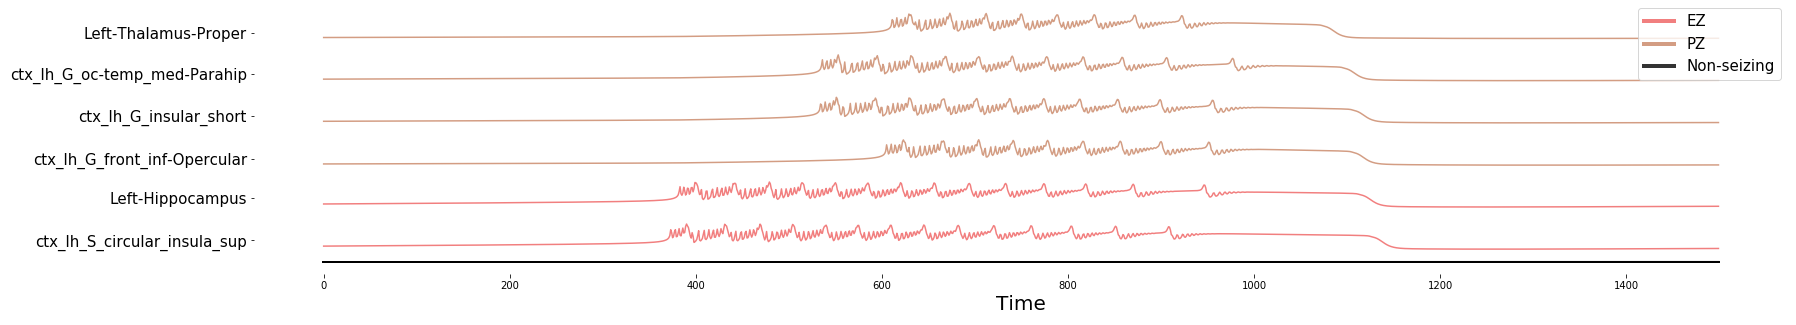
\includegraphics[width=\textwidth]{figures/source_activity_syn_data.png}
    \caption{Source activity}
  \end{subfigure}
  \begin{subfigure}{\linewidth}
    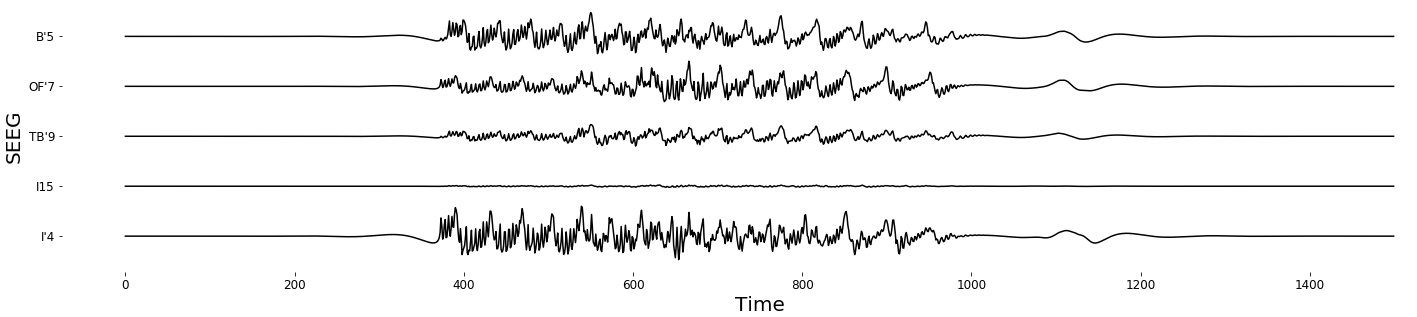
\includegraphics[width=\textwidth]{figures/seeg_syn_data.png}
    \caption{SEEG activity}
  \end{subfigure}
  \caption{Simulated seizure propagation pattern}
  \label{fig:syn-data}
\end{figure}
\subsection*{Modeled data features}
Given appropriate parameter values 2D Epileptor can capture some of the important characteristics of a seizure namely seizure onset and seizure length, which are sufficient for the purposes of identifying spatio-temporal seizure propagation patterns. Log. SEEG power encompasses both these features and hence forms a good candidate data feature that can be modeled using 2D Epileptor. Figure \ref{fig:data-features} shows the features extracted from synthetic dataset shown in figure \ref{fig:syn-data}

\begin{figure}[h!]
  \centering
  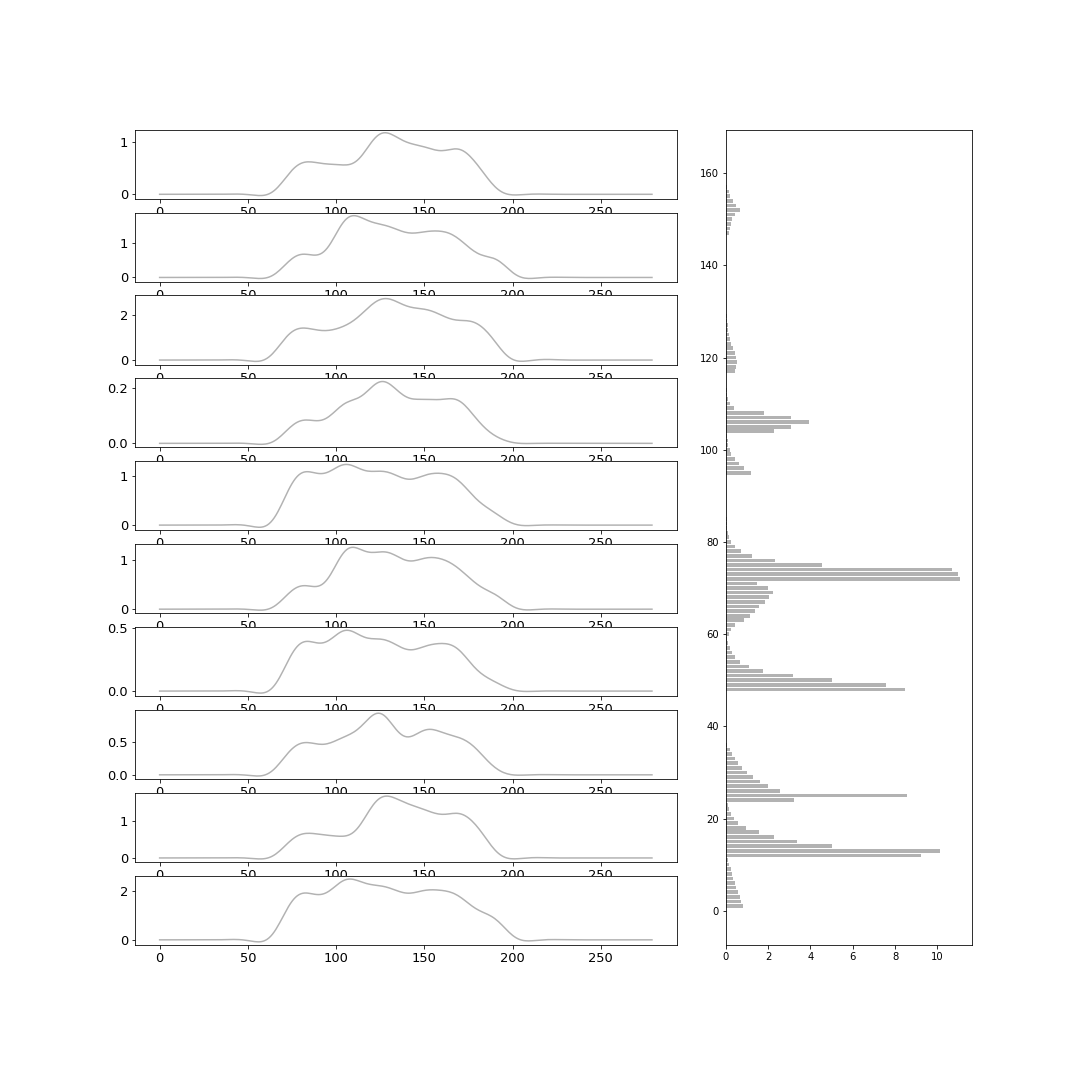
\includegraphics[width=\textwidth]{figures/modelled_data_features.png}
  \caption{Modeled data features. SEEG log power of 10 sensors(left) and total power per sensor(right)}
  \label{fig:data-features}
\end{figure}
\FloatBarrier
\section*{Model}
The dependency structure between parameters of virtual epileptic patient(VEP) model is shown in figure \ref{fig:vep_model}
\begin{figure}
  \centering
  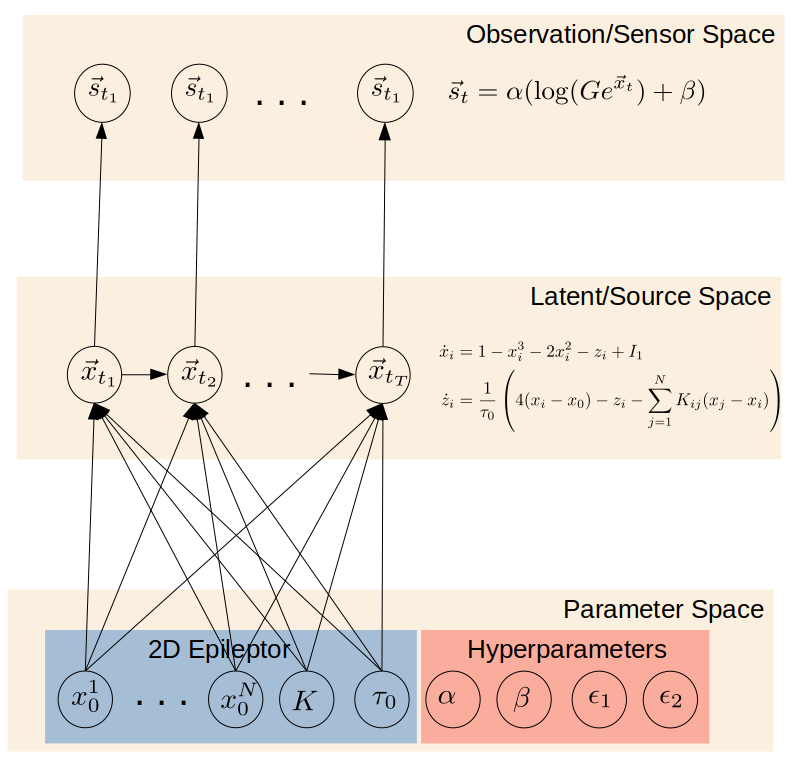
\includegraphics[width=\textwidth]{figures/vep_model.png}
  \caption{Probabilistic graphical model of virtual epileptic patient}
  \label{fig:vep_model}
\end{figure}
\begin{align*}
  P(\theta, \textbf{X} | \textbf{D}) & \propto P(\textbf{D} | \theta, \textbf{X}) P(\textbf{X}, \theta) \\
  \text{where}, \\
  \textbf{D} & = (\textbf{S}, \vec \rho), \textbf{S} = \text{Log SEEG power}, \vec \rho=\text{Total power in each sensor} \\ 
  \textbf{S} & =
               \begin{pmatrix}
                 s_{t_1}^1 & s_{t_1}^2 & \cdots & s_{t_1}^M \\
                 s_{t_2}^1 & s_{t_2}^2 & \cdots & s_{t_2}^M \\
                 \vdots & \vdots & \ddots & \vdots \\
                 s_{t_T}^1 & s_{t_T}^2 & \cdots & s_{t_T}^M \\
               \end{pmatrix}_{T \times M}
  \textbf{X}  =
  \begin{pmatrix}
    x_{t_1}^1 & x_{t_2}^1 & \cdots & x_{t_T}^1 \\
    x_{t_1}^2 & x_{t_2}^2 & \cdots & x_{t_T}^2 \\
    \vdots & \vdots & \ddots & \vdots \\
    x_{t_1}^N & x_{t_2}^N & \cdots & x_{t_T}^N \\
  \end{pmatrix}_{N \times T} \\
  \theta & = (\vec x_0, k, \tau_0, \alpha, \beta) \\
\end{align*}

\subsection*{\textit{Likelihood}}
\begin{align*}
  P(\textbf{S}, \rho | \textbf{X}, \theta) & = P(\textbf{S} | \textbf{X}, \theta) P(\rho | \textbf{S}, \theta) \\
  P(\textbf{S} | \textbf{X}, \theta) & = \prod_{i=1}^{M} \prod_{j=1}^{T}P(s_{t_j}^{i} | \vec x_{t_j}, \theta) \\ 
  P(s_{t}^{i} | \vec x_{t}, \theta) & \sim  \mathcal{N}(\alpha (\log \langle G_i\,, e^{\vec x_t} \rangle + \beta), \epsilon_1), \text{where}, \\
                                           & \text{$G$ is a projection matrix from source space to sensor space}  \\
  P(\vec \rho^i | \textbf{S}, \theta) & \sim \prod_{i=1}^{M}\mathcal{N}(\frac{1}{T}\sum_{j=1}^T(s_{t_j}^i)^2, \epsilon_2)  \\
\end{align*}
% 
\subsection*{\textit{Priors}}
Source dynamics are assumed to follow trajectories given by 2D Epileptor
\begin{align*}
  \dot x_i &= 1 - x_i^3 - 2 x_i^2 - z_i + I_1\\
  \dot z_i & = \frac{1}{\tau_0} \left( 4(x_i - x_0) - z_i - \sum_{j=1}^{N}K_{ij}(x_j - x_i)\right) \\
\end{align*}

\begin{align*}
  P(\theta, \textbf{X}) & = P(\textbf{X} | \theta) P(\theta) \\
  P(\textbf{X} | \theta) & = P(\vec x_{t_1} | \theta)\prod_{j=2}^{T}P(\vec x_{t_j} | \vec x_{t_{j-1}}, \theta) \\
  P(\vec x_{t_j} | \vec x_{t_{j-1}}, \theta) & = \delta(x_{t_j} - f(x_{t_{j-1}}, \theta)) \\
  f(x_{t_{j-1}}, \theta)) & = x_{t_{j-1}} + dt \dot x \\
  P(\theta) & = P(x_0, K, \tau_0, \alpha, \beta) \\
                        & = P(x_0)P(K)P(\tau_0)P(\alpha)P(\beta)\\
\end{align*}

Prior distributions of all inferred parameters are given in table \ref{tab:priors}

\begin{table}
  \centering
  $\begin{array}{|c|c|}
     \hline
     Parameter & Prior \\
     \hline
     x_0^i & \mathcal{N}(\mu_{x_0}^i, 1) \\
     K & \mathcal{N}(1, 10) \\
     \tau_0 & \mathcal{N}(20, 10) \\
     \alpha & \mathcal{N}(1, 10) \\
     \beta & \mathcal{N}(0, 10) \\
     \epsilon_1 & \mathcal{N}(1, 10) \\
     \epsilon_2 & \mathcal{N}(1, 10) \\
     \hline
   \end{array}$  
   \caption{Prior distributions of all inferred parameters}
   \label{tab:priors}
 \end{table}


 \section*{Results}
 NUTS parameters across iterations and pair plots for inferred scalar parameters from 4 chains are shown in figures \ref{fig:nuts_diags_chain1} - \ref{fig:nuts_diags_chain4}.

 \textit{sampler parameters:}
 
 \begin{tabular}{lcc}
   No. of warmup iterations & : & 200 \\
   No. of sampling iterations & : & 200 \\
   Target acceptance statistic ($\delta$) & : & 0.9 \\
   Max. tree depth & : & 10 \\
   Metric & : & diagonal \\
 \end{tabular}

 \clearpage
 \textbf{Problems}: 
 \begin{itemize}
 \item Inference works well when the observations are at source space but fails when observations are in sensor space. 
 \item All chains hit max. tree depth
 \item Sampling is very slow, it takes 3-4 days to finish 200 warmup + 200 sampling itearations
 \item Fixing observation noise($\epsilon_1=1, \epsilon_2=1$) causes many divergent transitions in all chains
 \end{itemize}
 

Some diagnostics from cmdstan \textit{diagnose} utility:

\begin{lstlisting}[breaklines]
 789 of 1600 (49%) transitions hit the maximum treedepth limit of 10, or 2^10 leapfrog steps. Trajectories that are prematurely terminated due to this limit will result in slow exploration and you should increase the limit to ensure optimal performance.

 8 of 1600 (0.5%) transitions ended with a divergence.  These divergent transitions indicate that HMC is not fully able to explore the posterior distribution.  Try rerunning with adapt delta set to a larger value and see if the divergences vanish.  If increasing adapt delta towards 1 does not remove the divergences then you will likely need to reparameterize your model.

 The E-BFMI, 0.0049, is below the nominal threshold of 0.3 which suggests that HMC may have trouble exploring the target distribution.  You should consider any reparameterizations if possible.

 The following parameters had split R-hat greater than 1.1:
 Almost all the parameters
\end{lstlisting}
 
 \begin{figure}[h!]
   \centering
   \begin{subfigure}{1.0\linewidth}
     \includegraphics[width=\textwidth]{../results/hmc_debug/hmc/figures/nuts_diagnostics_syn_hmc_chain4.png}
   \end{subfigure}
   \begin{subfigure}{1.0\linewidth}
     \includegraphics[width=\textwidth]{../results/hmc_debug/hmc/figures/params_pair_plots_syn_hmc_chain4.png}
   \end{subfigure}
   \caption{Chain 1}
   \label{fig:nuts_diags_chain1}
 \end{figure}
 \begin{figure}[h!]
   \centering
   \begin{subfigure}{1.0\linewidth}
     \includegraphics[width=\textwidth]{../results/hmc_debug/hmc/figures/nuts_diagnostics_syn_hmc_chain1.png}
   \end{subfigure}
   \begin{subfigure}{1.0\linewidth}
     \includegraphics[width=\textwidth]{../results/hmc_debug/hmc/figures/params_pair_plots_syn_hmc_chain1.png}
   \end{subfigure}
   \caption{Chain 2}
   \label{fig:nuts_diags_chain2}
 \end{figure}
 \begin{figure}[h!]
   \centering
   \begin{subfigure}{1.0\linewidth}
     \includegraphics[width=\textwidth]{../results/hmc_debug/hmc/figures/nuts_diagnostics_syn_hmc_chain3.png}
   \end{subfigure}
   \begin{subfigure}{1.0\linewidth}
     \includegraphics[width=\textwidth]{../results/hmc_debug/hmc/figures/params_pair_plots_syn_hmc_chain3.png}
   \end{subfigure}
   \caption{Chain 3}
   \label{fig:nuts_diags_chain3}
 \end{figure}
 \begin{figure}[h!]
   \centering
   \begin{subfigure}{1.0\linewidth}
     \includegraphics[width=\textwidth]{../results/hmc_debug/hmc/figures/nuts_diagnostics_syn_hmc_chain2.png}
   \end{subfigure}
   \begin{subfigure}{1.0\linewidth}
     \includegraphics[width=\textwidth]{../results/hmc_debug/hmc/figures/params_pair_plots_syn_hmc_chain2.png}
   \end{subfigure}
   \caption{Chain 4}
   \label{fig:nuts_diags_chain4}
 \end{figure}
\end{document}

